%% Recipes_Detector.tex
%% Created:     Tue Apr  4 16:37:17 2017 by Koehler@I-Mac
%% Last change: 2020-09-04
%%
%% subsection for Detector Recipes
%%
%%%%%%%%%%%%%%%%%%%%%%%%%%%%%%%%%%%%%%%%%%%%%%%%%%%%%%%%%%%%%%%%%%%%%%%%%%%%%
\subsection{Detector calibration recipes}
\label{Sec:detector_calibration}

METIS will have three focal plane detector arrays:
\begin{itemize}
\item One $2\mathrm{k}\times 2\mathrm{k}$ HAWAII2RG detector used for
  LM-band imaging and slit spectroscopy.
\item One $2\mathrm{k}\times 2\mathrm{k}$ GeoSnap (Teledyne) detector
  used for N-band imaging and slit spectroscopy.
\item An array of four $2\mathrm{k}\times 2\mathrm{k}$ HAWAII2RG
  detectors used for LM-band integral-field spectroscopy.
\end{itemize}
This section lists recipes that calibrate detector characteristics
independent of a specific instrument mode. Where \FITS{_det} appears
in FITS keywords of input or product files, it is taken to mean
\FITS{_LM}, \FITS{_N} or \FITS{_IFU} according to the detector
array for which data are being processed.

\subsubsection{Detector linearity and gain determination recipe \REC{metis_det_lingain}}
\label{sssec:metis_det_lingain}
\label{rec:metis_det_lingain}
\label{rec:metisdetlingain}

The recipe \REC{metis_det_lingain} determines detector (non-)linearity and absolute detector
gain from a set of flat-field frames taken with the broad-band lamp
over a range of detector exposure times (DITs) and flux levels. The
recipe structure will be similar as for \CODE{detmon_ir_lg} % Not a \REC because it is not our recipe
\cite{detmon-manual}; however, further insight into detector behaviour
(in particular of GeoSnap) may necessitate development of more complex
procedures.

The linearity curve is given by the measured background level as a
function of exposure time for constant illumination. For each pixel
the coefficients of a polynomial fit (order TBD) will be recorded in a
coefficient cube, which can in turn be used to correct for
non-linearity in other recipes. Pixels whose coefficients differ
significantly from the majority of pixels will be marked as bad.

Detector gain is typically computed pixelwise as the slope of a linear
fit of the variance against the mean (or median) values over a set of
frames taken over a range of DITs and illumination levels.  For
mid-infrared detectors that suffer from \ac{ELFN}, e.g.\ the AQUARIUS
detector, this approach does not work.  The GeoSnap is not expected to
show \ac{ELFN}, hence gain determination is probably possible.

The set of calibration frames used for this recipes will include
exposures with WCU window closed (\CODE{LAMP OFF}), which will be used
as `dark' frames that captur thermal emission within the
instrument. This is subtracted from all other exposures in the
sequence.

This satisfies \REQ{METIS-5997}.

\newpage
\begin{recipedef}
  Name:                & \hyperref[rec:metis_det_lingain]{\REC{metis_det_lingain}}                                                             \\
  Purpose:             & determine non-linearity and gain of the detectors                                   \\
  Requirements:        & \REQ{METIS-5997}                                                                    \\
  Type:                & Calibration                                                                         \\
  Templates:           & \TPL{METIS_img_lm_cal_DetLin}                                                       \\
                       & \TPL{METIS_img_n_cal_DetLin}                                                        \\
                       & \TPL{METIS_ifu_cal_DetLin}                                                          \\
  Input data:          & \hyperref[dataitem:detlin_det_raw]{\RAW{DETLIN_det_RAW}}: (set of \FITS{FLAT,LAMP} frames taken with increasing DIT) \\
                       & \hyperref[dataitem:dark_internal_det_raw]{\RAW{DARK_INTERNAL_det_RAW}}: (set of internal darks taken at the start of the template) \\
  Matched keywords:    & Subsystem ID \TODO{TBD}                                                             \\
  Algorithm:           & Subtract instrument dark (\CODE{hdrl_imagelist_sub_image}).                         \\
                       & Compute mean and variance for each frame (\CODE{TBD}).                              \\
                       & Gain is determined as the slope of variance against mean (\hyperref[drl:metis_derive_gain]{\DRL{metis_derive_gain}}) \\
                       & Fit polynomial of value as a function of DIT and illumination level for each pixel (\hyperref[drl:metis_derive_nonlinearity]{\CODE{metis_derive_nonlinearity}}). \\
                       & Flag pixels with coefficients significantly different from the mean of all pixels. (\CODE{hdrl_bpm_fit_compute}) \\
  Output data:         & \hyperref[dataitem:gain_map_det]{\PROD{GAIN_MAP_det}}                                    \\
                       & \hyperref[dataitem:linearity_det]{\PROD{LINEARITY_det}}                                 \\
                       & \hyperref[dataitem:badpix_map_det]{\PROD{BADPIX_MAP_det}}                                \\
  Expected accuracies: & \TODO{TBD}                                                                          \\
  QC1 parameters:      & \hyperref[qc:qc_lin_gain_mean]{\QC{QC LIN GAIN MEAN}}                                    \\
                       & \hyperref[qc:qc_lin_gain_rms]{\QC{QC LIN GAIN RMS}}                                      \\
                       & \hyperref[qc:qc_lin_num_badpix]{\QC{QC LIN NUM BADPIX}}                                  \\
  hdrl functions:      & \CODE{hdrl_imagelist_sub_image}                                                     \\
                       & \CODE{hdrl_bpm_fit_compute}                                                         \\
\end{recipedef}

\begin{figure}[hb]
  \centering
  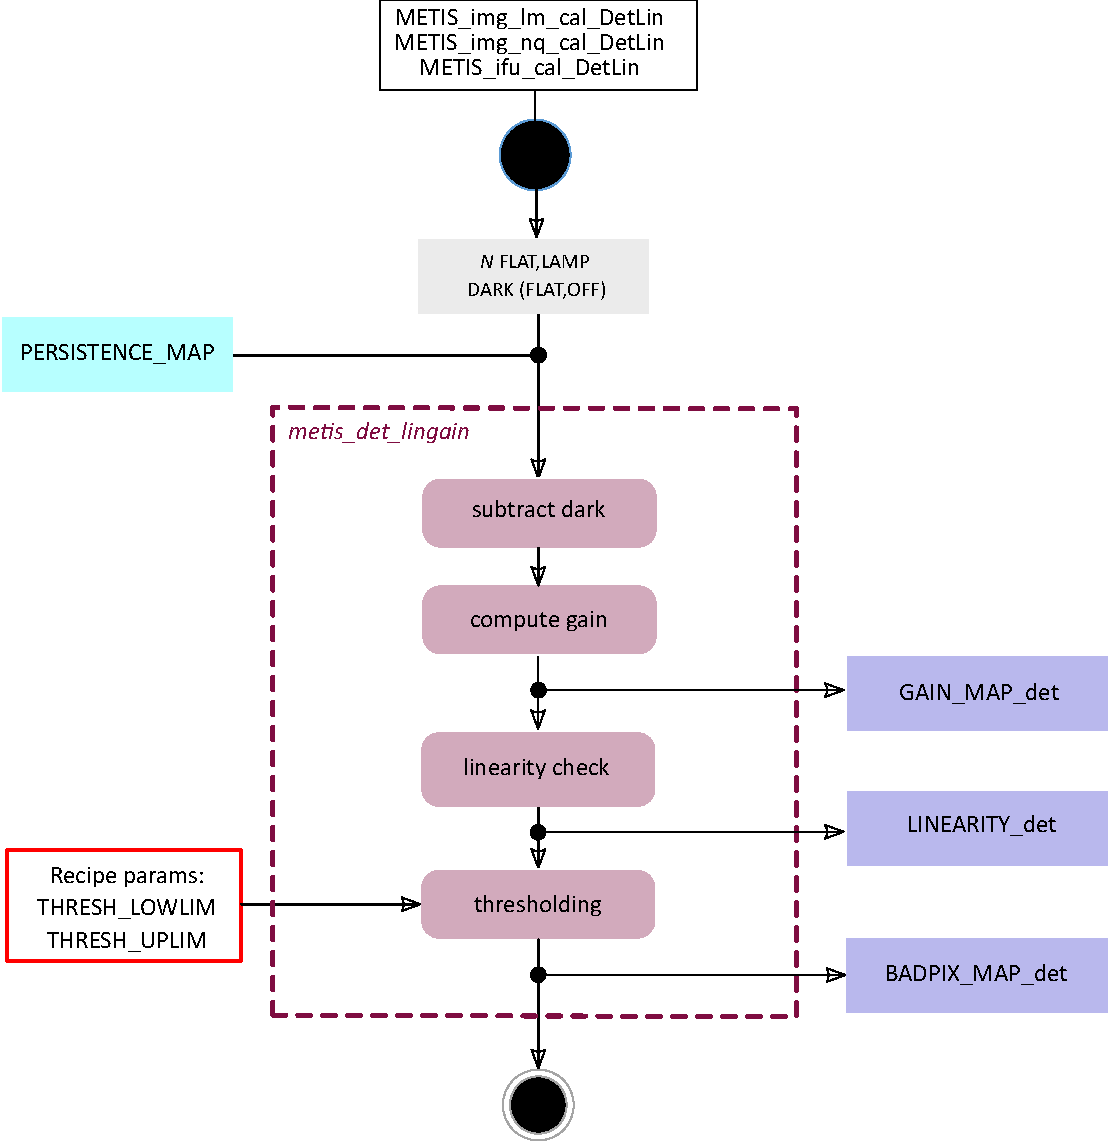
\includegraphics[width=0.65\textwidth]{metis_det_lingain}
  \caption[Recipe: \REC{metis_det_lingain}]{\REC{metis_det_lingain} --
    determination of linearity and gain of the detectors.}
  \label{Fig:rec_det_lingain}
\end{figure}


\clearpage

\subsubsection{Master dark recipe \REC{metis_det_dark}}
\label{sssec:metis_det_dark}
\label{rec:det_dark}
\label{rec:metis_det_dark}

Darks are taken in daytime for all science detectors
\cite{METIS-calibration_plan}. The data will be classified by detector
(e.g.~\FITS{DET.ID} and \FITS{DET.CHIP.ID}) and integration time
(\FITS{DET.DIT}).\footnote{The dark current is not expected to depend on the readout mode of the detectors. Should hardware tests reveal such a dependence, the recipe will be amended to classify on readout mode as well.} There will be ``METIS-dark''
(with the CLOSED position of the CFO-PP1 wheel) and ``Imager-dark''
(with the CLOSED position in the subsystem PP1), to be distinguished
by keyword \TBD. The former will be used for pipeline processing, the
latter for monitoring purposes.

Each set of raw dark frames is processed into a master dark. For the
IFU, both raw frames and master dark have four extensions
corresponding to the four detectors in the focal-plane array. The
recipe also produces bad pixel masks by identifying hot pixels whose
dark current differs significantly (by more than $\pm 5\sigma$) from
the average over the detector.

This fulfills \REQ{METIS-6063}.

\begin{recipedef}
  Name:                & \hyperref[rec:metis_det_dark]{\REC{metis_det_dark}}                                                        \\
  Purpose:             & determine the dark current of the detectors                                 \\
  Requirements:        & \REQ{METIS-6063}                                                            \\
  Type:                & Calibration                                                                 \\
  Templates:           & \TPL{METIS_gen_cal_dark}                                                    \\
  Input data:          & \hyperref[dataitem:linearity_det]{\STATCALIB{LINEARITY_det}}  \\
                       & \hyperref[dataitem:persistence_map]{\EXTCALIB{PERSISTENCE_MAP}}  \\
                       & \hyperref[dataitem:dark_det_raw]{\EXTCALIB{DARK_det_RAW}}  \\
  Parameters:          & Combination method (\texttt{median}, \texttt{mean},
                         \texttt{sigclip},\dots)                                                  \\
                       & Parameters for combination methods                                          \\
                       & Thresholds for deviant-pixel identification                                      \\
  Algorithm:           & Group files by detector and \texttt{DIT}, based on header keywords           \\
                       & Call function \DRL{metis_determine_dark} for each set of files\\
                       & Compute median or average of input frames to improve statistics.            \\  % separate routine, or part of determine dark
                       & call \DRL{metis_update_dark_mask} to flag deviant pixels \\
  Output data:         & \hyperref[dataitem:master_dark_det]{\PROD{MASTER_DARK_det}}                                                      \\
% The BPM_COLD_det and BPM_HOT_det do not seem to add value that BADPIX_MAP_det
% does not already provide. Furthermore, the COLD/HOT specific items are not
% otherwise used in the design, so it seems simpler to just remove them.
%                       & \hyperref[dataitem:bpm_cold_det]{\PROD{BPM_COLD_det}}                                                         \\
%                       & \hyperref[dataitem:bpm_hot_det]{\PROD{BPM_HOT_det}}                                                          \\
                       & \hyperref[dataitem:badpix_map_det]{\PROD{BADPIX_MAP_det}}                                                          \\
  Expected accuracies: & \TBD                                                                         \\
  QC1 parameters:      & \QC{QC DARK MEAN}                                                              \\
                       & \QC{QC DARK MEDIAN}                                                            \\
                       & \QC{QC DARK RMS}                                                               \\
                       & \QC{QC DARK NBADPIX}                                                             \\
                       & \QC{QC DARK NCOLDPIX}                                                               \\
                       & \QC{QC DARK NHOTPIX}                                                                \\
                       & (more \TBD)                                                                  \\
  hdrl functions:      & \CODE{hdrl_bpm_3d_compute}                                 \\
                       & \CODE{hdrl_imagelist_collapse}                             \\
\end{recipedef}

\begin{figure}[hb]
  \centering
  \includegraphics[width=0.5\textwidth]{figures/metis_det_dark_v0.83.pdf}  % RemarK. The original file: figures/metis_det_dark.pdf is still available
  \caption[Recipe: \REC{metis_det_dark}]{\REC{metis_det_dark} -- creation of master
    dark and bad pixel maps}
  \label{Fig:rec_det_dark}
\end{figure}

\clearpage

\subsubsection{Persistence map creation recipe \REC{metis_det_persistence}}
\label{sssec:metis_det_persistence}

Infrared detectors are prone to persistence due to charges trapped on a
variety of timescales. The correction for a given science or
calibration exposure is built from a sequence of exposures preceding
the exposure in question. As these may include exposures taken for
another proprietary programme, the recipe is run by ESO on data taken
from the science archive and its products are again ingested into the
archive. 

\begin{recipedef}\label{rec:metis_det_persistence}
  Name:                & \hyperref[rec:metis_det_persistence]{\REC{metis_det_persistence}}           \\
  Purpose:             & compute persistence correction maps        \\
  Requirements:        & \REQ{METIS-9145}                      \\
  Type:                & Calibration                           \\
  Templates:           & --                                    \\
  Parameters:          & \TBD                                  \\
  Algorithm:           & see hdrl functions:                   \\
  Output data:         & \hyperref[dataitem:persistence_map]{\PROD{PERSISTENCE_MAP}}                \\
  Expected accuracies: & \TBD                                  \\
  QC1 parameters:      & see hdrl functions:                   \\
  hdrl functions:      & \TBD (\CODE{hdrl_persistence_compute} \\
\end{recipedef}

\begin{figure}[hb]
  \centering
  \resizebox{0.6\textwidth}{0.1\textwidth}{\TODO{\fbox{Figure to be done}}}
  \caption[Recipe:
  \REC{metis_det_persistence}]{\REC{metis_det_persistence} -- creation
    of persistence correction frames.}
  \label{Fig:rec_det_persistence}
\end{figure}

%%%%%%%%%%%%%%%%%%%%%%%%%%%%%%%%%%%%%%%%%%%%%%%%%%%%%%%



%%% Local Variables:
%%% TeX-master: "METIS_DRLD"
%%% End:
